\subsection{État du jeu}
\begin{frame}{État du jeu}
	{\texttt{*} signifie constant} % Ça fait bizarre là où c'est mais ça gêne pas
	\begin{columns}
		\begin{column}{0.5\textwidth}
			\begin{typeag}{Personnage}
				\variable{vies}{entier}\\
				\variable{positionX}{entier}\\
				\variable{positionY}{entier}\\
				\variable{vitesse}{entier*}
			\end{typeag}
			\begin{typeag}{Champignon}
				\variable{vie}{Champignon[nb[max]}\\
				\variable{estVénéneux}{booléen}\\
				\variable{positionX}{entier}
				\variable{positionY}{entier}

			\end{typeag}
			
		\end{column}
		\begin{column}{0.5\textwidth}
			\begin{typeag}{Zone de jeu}
				\variablei{champis}{Champignon[nb[max]}\\
				\variablei{tir}{Projectile}\\
				\variablei{couleurs}{entier}
				\variablei{score}{entier}
				\variablei{niveau}{entier}
			\end{typeag}
			\begin{typeag}{Segment}
				\variable{etat}{entier}\\
				\variable{vitesse}{entier}\\
				\variable{direction}{entier}
				\variable{positionX}{entier}
				\variable{positionY}{entier}
			\end{typeag}
		\end{column}
	\end{columns}
\end{frame}

\subsection{Configuration initiale du jeu}
\begin{frame}{Configuration initiale du jeu}
	\begin{typeag}{Projectile}
		\variablei{actif}{2}\\
		\variable{vitesse}{entier}
		\variablei{positionX}{largeurEcran/2}\\
		\variablei{positionY}{hauteurEcran-hauteurPersonnage}
	\end{typeag}
	\begin{typeag}{Ennemi}
		\variablei{type}{entier}\\
		\variablei{vitesse}{entier}
		\variablei{direction}{entier}
		\variablei{positionX}{entier ou réel}\\
		\variablei{positionY}{entier ou réel}
	\end{typeag}
\end{frame}

\subsection{Évolution de l'état du jeu}
\begin{frame}{Entrées du joueur}
	\begin{columns}
		\begin{column}{0.4\textwidth}
			\begin{block}{Déplacement}
				Restreint :
				
				\smallskip
				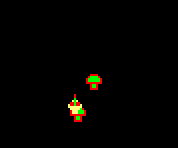
\includegraphics[width=\textwidth]{imgs/collisionChampignon.png}
			\end{block}
		\end{column}
		\begin{column}{0.4\textwidth}
			\begin{block}{Tir}
				Unique et libre :
				
				\smallskip
				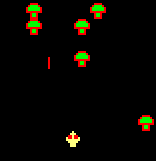
\includegraphics[width=\textwidth]{imgs/tirEtDeplacement.png}
			\end{block}
		\end{column}
	\end{columns}
\end{frame}
\begin{frame}{Évolution des éléments}
	\begin{columns}
		\begin{column}{0.3\textwidth}
			\begin{block}{Mort du joueur}
				Instantanée pour tout ennemi :
				
				\smallskip
				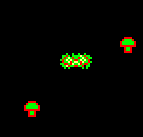
\includegraphics[width=\textwidth]{imgs/mortNain.png}
			\end{block}
		\end{column}
		\begin{column}{0.3\textwidth}
			\begin{block}{Tir/Ennemi}
				Destruction instantanée :
				
				\smallskip
				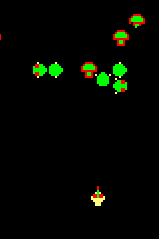
\includegraphics[width=\textwidth]{imgs/destructionSegment.png}
			\end{block}
		\end{column}
		\begin{column}{0.3\textwidth}
			\begin{block}{Champignons}
				Destructibles mais gênants pour le joueur et le centipède :
				
				\smallskip
				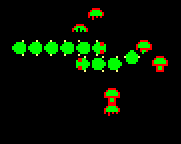
\includegraphics[width=\textwidth]{imgs/champignonsEtCentipede.png}
			\end{block}
		\end{column}
	\end{columns}
\end{frame}
